% Fig. 3 -- ablation on authored144. Data: mean_family_balanced_accuracy from
%   bench/results/authored144-Qwen3-0.6B-ONNX-q4f16-readout-shots0.json            0.38498
%   bench/results/authored144-Qwen3-0.6B-ONNX-q4f16-readout-shots3.json            0.41937
%   bench/results/authored144-Qwen3-0.6B-ONNX-q4f16-generate-shots3.json           0.41937
%   bench/results/authored144-Qwen3-0.6B-ONNX-q4f16-readout-full-shots3.json       0.44164
%   bench/results/authored144-Qwen3-0.6B-ONNX-q4f16-readout-calibrated-shots3.json 0.45948
%   bench/results/authored144-Qwen3-0.6B-ONNX-q4f16-readout-cyclic-shots3.json     0.48276
% Reference lines: chance = 1/3; 0.440 and 0.813 are PUBLISHED by openjev
% (reference-openjev/results/raw/browser-model-ladder.json), not measured here.
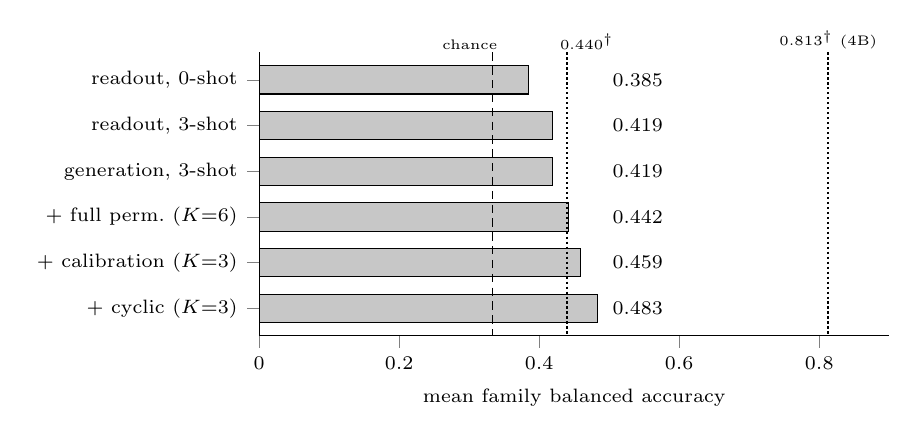
\begin{tikzpicture}
\begin{axis}[
    xbar, scale only axis, width=0.66\columnwidth, height=36mm,
    xmin=0, xmax=0.9, ymin=0.4, ymax=6.6, y dir=reverse,
    bar width=3.6mm,
    ytick={1,2,3,4,5,6},
    yticklabels={{readout, 0-shot},{readout, 3-shot},{generation, 3-shot},{+ full perm.\ ($K{=}6$)},{+ calibration ($K{=}3$)},{+ cyclic ($K{=}3$)}},
    yticklabel style={font=\scriptsize}, xticklabel style={font=\scriptsize},
    xlabel={mean family balanced accuracy}, xlabel style={font=\scriptsize},
    xtick={0,0.2,0.4,0.6,0.8},
    axis lines*=left, tick align=outside, clip=false]
  \addplot[draw=black, fill=black!22] coordinates {(0.38498,1) (0.41937,2) (0.41937,3) (0.44164,4) (0.45948,5) (0.48276,6)};
  % value labels, placed right of every bar and clear of the reference lines
  \node[font=\scriptsize, anchor=west, inner sep=1pt] at (axis cs:0.50,1) {0.385};
  \node[font=\scriptsize, anchor=west, inner sep=1pt] at (axis cs:0.50,2) {0.419};
  \node[font=\scriptsize, anchor=west, inner sep=1pt] at (axis cs:0.50,3) {0.419};
  \node[font=\scriptsize, anchor=west, inner sep=1pt] at (axis cs:0.50,4) {0.442};
  \node[font=\scriptsize, anchor=west, inner sep=1pt] at (axis cs:0.50,5) {0.459};
  \node[font=\scriptsize, anchor=west, inner sep=1pt] at (axis cs:0.50,6) {0.483};
  \draw[densely dashed] (axis cs:0.3333,0.4) -- (axis cs:0.3333,6.6);
  \draw[densely dotted, thick] (axis cs:0.440,0.4) -- (axis cs:0.440,6.6);
  \draw[densely dotted, thick] (axis cs:0.813,0.4) -- (axis cs:0.813,6.6);
  \node[font=\tiny, anchor=south east, inner sep=1pt] at (axis cs:0.345,0.4) {chance};
  \node[font=\tiny, anchor=south west, inner sep=1pt] at (axis cs:0.425,0.4) {0.440$^{\dagger}$};
  \node[font=\tiny, anchor=south, inner sep=1pt] at (axis cs:0.813,0.4) {0.813$^{\dagger}$ (4B)};
\end{axis}
\end{tikzpicture}
